%==============================================================================
% short introduction to get template running on WINDOWS
% further explanation can be found in the pptx
% can be removed after first compilation 
%
% install MikTeX (http://www.miktex.org) - activate auto-install of packages
% install ActivePerl (https://www.perl.org/) - add to HOME
% system reboot
%
% use command-line or IDE in admin-mode to execute the  following commands
% in the specified order (pdflatex used because we want the PDF in the end)
% 
%
% After changes in glossary you need to execute the following command 
% to use the new acronyms
%
% pdflatex bt_engbrocks.tex
% makeglossaries bt_engbrocks
% pdflatex bt_engbrocks.tex
% bibtex bt_engbrocks
% pdflatex bt_engbrocks.tex
% pdflatex bt_engbrocks.tex
%
% After changes in literature you need to execute the following command
% to use the new reference
%
% bibtex bt_engbrocks
%
%==============================================================================

%==============================================================================
% Moved here from header to be compatible with the VSCode Extension: Latex Workshop
\documentclass[
	pdftex,				% PDFTex verwenden da ausschliesslich ein PDF erzeugt wird.
	a4paper, %twoside,	% Verwenden von DIN A4 Papier.
	11pt,				% Grosse Schrift, besser geeignet für A4.
	parskip=half,		% Halbe Zeile Abstand zwischen Absätzen.
	numbers=noenddot,	% Keine Punkte hinter Nummern
	pagesize,           % Schreibt die Papiergroesse in die Datei 
	BCOR=10mm,			% Bindekorrektur
	DIV=13,				% Alternativ 12 oder 14
	headinclude,		% Kopfzeile in den Textbereich
	headsepline,		% Linie nach Kopfzeile.
	titlepage,
	headings=small,
	bibliography=totocnumbered,	% Bibliographie im TOC nummeriert
]{scrbook}
%==============================================================================


%==============================================================================
% Dokument einrichten und Pakete laden
%==============================================================================

\usepackage{setspace}\setstretch{1.2} 
%\usepackage{titlesec}
\usepackage{longtable}

%\titlespacing\section{0pt}{12pt plus 4pt minus 2pt}{0pt plus 2pt minus 2pt}
%\titlespacing\subsection{0pt}{12pt plus 4pt minus 2pt}{0pt plus 2pt minus 2pt}
%\titlespacing\subsubsection{0pt}{12pt plus 4pt minus 2pt}{0pt plus 2pt minus 2pt}

\usepackage{scrhack}
\usepackage{tabularx}

\usepackage[printonlyused]{acronym}
\usepackage{multicol}

\usepackage[table]{xcolor}

\usepackage{comment}

%
% Zeichenkodieruung und Sprache
%

\usepackage[utf8]{inputenc} % Dokument
\usepackage[T1]{fontenc} % Schrift
\usepackage[ngerman, english]{babel}

\usepackage{eurosym}

%
% PDF-Metadaten setzen
%

\usepackage{pdfpages}
\usepackage[
	% Titel des PDF Dokuments
	pdftitle={BT Engbrocks: Development of a Concept for the Monitoring of Decentralized Identity Solutions Based on DevOps Concepts},
	% Autor des PDF Dokuments
	pdfauthor={Tim Engbrocks},
	% Thema des PDF Dokuments
	pdfsubject={Bachelor thesis},
	% Erzeuger des PDF Dokuments
	pdfcreator={Tim Engbrocks},
	% Schlüsselwörter für das PDF
	pdfkeywords={},
	% Dokumenttitel statt Dateiname anzeigen
	pdfdisplaydoctitle=true,																% Sprache des Dokuments
	pdflang=en,
	bookmarksopen=true,
	bookmarksdepth=1,
	colorlinks,
	linkcolor = black,
	citecolor=black,
	urlcolor=black,
]{hyperref}

%
%  Zusätzliche Pakete laden
%

% Anführungszeichen
\usepackage[style=american]{csquotes}

% erweiterte Tabelleneigenschaftn
\usepackage{array, ragged2e}

% Einbinden von Grafiken
\usepackage{graphicx}	

% mathematischer Textsatz
%\usepackage{amsmath}
%\usepackage{amssymb}
%\usepackage{dsfont}

% Textteile drehen
%\usepackage{rotating}	

% Farbpakete
%\usepackage{color}

% Quellcode sauber formatieren
\usepackage{listings}	

% Font 'Latin Modern Family' verwenden
\usepackage{microtype}
\usepackage{helvet}
\usepackage{mathptmx}

%==============================================================================
% Einstellungen und Definitionen
%==============================================================================

% Farben definieren

\definecolor{light-gray}{gray}{0.95}
%\definecolor{LinkColor}{rgb}{0,0,0.5}
%\definecolor{ListingBackground}{rgb}{0.85,0.85,0.85}
%\definecolor{CommentColor}{rgb}{0, 0.5, 0}
%\definecolor{StringColor}{rgb}{0.63, 0.09, 0.09}

% KOMA-Script Option, Zeilenumbruch bei Bildbeschreibungen.
\setcapindent{1em}

% Stil der Kopf- und Fusszeilen.
\usepackage[headsepline,automark,pagestyleset=KOMA-Script, markcase=ignoreuppercase]{scrlayer-scrpage}
\pagestyle{scrheadings}

% Stil der Überschriften auf normale Schrift.

%\setkomafont{sectioning}{\normalfont\bfseries}		 % Titel mit Normalschrift
\setkomafont{captionlabel}{\normalfont\bfseries}	 % Fette Beschriftungen 
%\setkomafont{pageheadfoot}{\normalfont\itshape}     % Kursive Seitentitel
\setkomafont{descriptionlabel}{\normalfont\bfseries} % Fette Beschreibungstitel

% Codelisting korrekt bezeichnet ausgeben
%\renewcommand\lstlistingname{Source code}

%==============================================================================
% Listings
%==============================================================================

\lstloadlanguages{% Check Dokumentation for further languages ...
  XML,
  HTML,
  Java,
  Tex
}


\lstset{
  %basicstyle=\scriptsize\ttfamily, % Standardschrift
	basicstyle=\footnotesize\ttfamily,
  %numbers=left, % Ort der Zeilennummern
  %numberstyle=\tiny, % Stil der Zeilennummern
  %stepnumber=2, % Abstand zwischen den Zeilennummern
	%numberblanklines=false,
  numbersep=5pt, % Abstand der Nummern zum Text
  tabsize=2, % Groesse von Tabs
  extendedchars=true, %
  breaklines=true, % Zeilen werden Umgebrochen
  %keywordstyle=\color{red},
  frame=b,
  % keywordstyle=[1]\textbf, % Stil der Keywords
  % keywordstyle=[2]\textbf, %
  % keywordstyle=[3]\textbf, %
  % keywordstyle=[4]\textbf, \sqrt{\sqrt{}} %
  %stringstyle=\color{white}\ttfamily, % Farbe der String
  showspaces=false, % Leerzeichen anzeigen ?
  showtabs=false, % Tabs anzeigen ?
  xleftmargin=17pt,
	xrightmargin=17pt,
  framexleftmargin=17pt,
  framexrightmargin=17pt,
  framexbottommargin=4pt,
  backgroundcolor=\color{white},
  showstringspaces=false % Leerzeichen in Strings anzeigen ?
}

\lstset{literate=%
    {Ö}{{\"O}}1
    {Ä}{{\"A}}1
    {Ü}{{\"U}}1
    {ß}{{\ss}}1
    {ü}{{\"u}}1 
    {ä}{{\"a}}1
    {ö}{{\"o}}1
    {~}{{\textasciitilde}}1
}

\usepackage{caption}
\DeclareCaptionFont{white}{\color{white}}
\DeclareCaptionFormat{listing}{\colorbox[cmyk] {0.43, 0.35, 0.35,0.01}{\parbox{\textwidth-2\fboxsep-2\fboxrule-0pt} {\hspace{15pt}#1#2#3}}}
\captionsetup[lstlisting]{format=plain, labelfont=bf}
%\captionsetup[lstlisting]{format=listing,labelfont=white, textfont=white,singlelinecheck=false, margin=0pt, font={bf,footnotesize}}

%
% code listing style
%

\lstdefinestyle{kit-cm}{
  backgroundcolor=\color{light-gray},
  belowcaptionskip=1\baselineskip,
  breaklines=true,
  frame=single,
  framexleftmargin=15pt,
  language=C,
  showstringspaces=false,
  basicstyle=\footnotesize\ttfamily, 
  numbers=left,                    
  numbersep=7pt,                
  numberstyle=\tiny\color{black},
  captionpos=b,
  keywordstyle=\color{blue}
}

\lstdefinelanguage{Swift}{
  keywords={associatedtype, class, deinit, enum, extension, func, import, init, inout, internal, let, operator, private, protocol, public, static, struct, subscript, typealias, var, break, case, continue, default, defer, do, else, fallthrough, for, guard, if, in, repeat, return, switch, where, while, as, catch, dynamicType, false, is, nil, rethrows, super, self, Self, throw, throws, true, try, associativity, convenience, dynamic, didSet, final, get, infix, indirect, lazy, left, mutating, none, nonmutating, optional, override, postfix, precedence, prefix, Protocol, required, right, set, Type, unowned, weak, willSet},
  ndkeywords={class, export, boolean, throw, implements, import, this},
  sensitive=false,
  comment=[l]{//},
  morecomment=[s]{/*}{*/},
  morestring=[b]',
  morestring=[b]"
}

\lstdefinelanguage{Gherkin}{
	morekeywords = {
		Given,
		When,
		Then,
		And,
		Scenario,
		Feature,
		But,
		Background,
		Scenario Outline,
		Examples
	},
	sensitive=true,
	morecomment=[l]{\#},
	morestring=[b]",
	morestring=[b]'
}


\lstdefinelanguage{json}{
     string=[s]{"}{"},
    stringstyle=\color{blue},
    comment=[l]{:},
    commentstyle=\color{black},
}

\DeclareCaptionFont{black}{\color{black}} 
\DeclareCaptionFormat{listing}
  {\colorbox{white}
     {\parbox{\dimexpr\textwidth-2\fboxsep}{\centering #1#2#3}}}
% \captionsetup[lstlisting]{format=listing,labelfont=black,textfont=black}

\usepackage{hyperref}
\usepackage{paralist}
\usepackage{subcaption}
\usepackage{booktabs}
\usepackage{listings}
\usepackage{caption}

%
% todo notes
%

\usepackage{todonotes}
%\usepackage[disable]{todonotes}	% hide all todo notes
%\presetkeys{todonotes}{inline}{}	% show all defined todos as inline

%
% glossary
%

%\usepackage[acronym,numberedsection,automake]{glossaries}
%\setacronymstyle{long-short}
%\loadglsentries{chapters/glossar.tex} %Removed because no more glossar needed
%\makeglossaries
%\glsdisablehyper
%
% load additional packages
%

\usepackage{calc}
\usepackage{enumitem}
\usepackage{multirow}
\usepackage{mathtools}
\usepackage{enumitem}
\usepackage{amsmath} 
\usepackage{amssymb}
\usepackage{wasysym}
\usepackage{rotating}
\usepackage{pgfplots}
\usepackage{longtable}
\usepackage{algorithm}
\usepackage{algpseudocode}
\usepackage{float}
\usepackage{pdfpages}
\usepackage{threeparttablex}
\usepackage{longtable,lscape}
\usepackage{tablefootnote}
\usetikzlibrary{patterns}
\usepackage{multicol}
\usepackage{bm}
\usepackage{esvect}
\floatname{algorithm}{Algorithmus}


\pgfplotsset{compat=1.16} 
\begin{document}

%==============================================================================

%
% add title pages
%

\frontmatter
\setcounter{secnumdepth}{3}
\begin{titlepage}
\thispagestyle{empty}
\enlargethispage{2cm}
%\enlargethispage{\baselineskip}

\sffamily
%\centering
\vspace*{-3.2cm}
\hspace*{-0.6cm}

\includegraphics[height=2.14cm]{figures/kit-logo.png}

\begin{addmargin}{4cm}

\vfill

\begin{tabular}{p{12cm}}
	{\bfseries\huge Bachelor Thesis}\\
	\\
	{Tim Engbrocks} \vspace{2em} \\
	\\
	{\linespread{0.85}\selectfont \Huge A DevOps-based Concept for the Monitoring of Decentralized Identity Solutions\par}   \vspace{0.5em}\\
	{\LARGE } \vspace{0.5em} \\
	{\LARGE }
\end{tabular}
\vfill
\vfill
\vfill


%\singlespacing

\vspace{1em}
\begin{tabular}{ll}
	
        
	May 2023 - September 2023 \\
	\\
	First referee: 				& Prof. Dr. Sebastian Abeck \\
	Second referee:				& Prof. Dr. Bernhard Neumair \\
	Supervising employee:		& Stefan Throner \\
	\\
	\multicolumn{2}{l}{Cooperation \& Management (C\&M, Prof. Abeck)} \\
	\multicolumn{2}{l}{Institute for Telematics, Department of Informatics} \\
	\multicolumn{2}{l}{www.cm.tm.kit.edu} \\
	\\
	\multicolumn{2}{l}{\scriptsize{KIT - The Research University in the Helmholtz Association}}\\
\end{tabular}

\end{addmargin}
\newpage
\thispagestyle{empty}
\end{titlepage}
\chapter*{Statement of Authorship}
%\addcontentsline{toc}{chapter}{Ehrenwörtliche Erklärung}
\thispagestyle{empty}

\vspace*{4cm}




I declare that I completed this thesis on my own and that information which has been directly or indirectly taken from other sources has been noted as such.
Neither this nor a similar work has been presented to an examination committee.

\bigskip
\bigskip
\bigskip

Karlsruhe, \today

\bigskip
\bigskip
\bigskip

\rule{0.3\textwidth}{0.4pt}\\
Tim Engbrocks
\cleardoublepage
\pdfbookmark[1]{Editing History}{toc}
\chapter*{Editing History}
\label{cha:history}

\newcolumntype{Y}{>{\centering\arraybackslash}X}

\begin{longtable}{ |p{2cm}|p{5.5cm}|p{6cm}|}
    \hline
           \textbf{Date} & \textbf{Section: Contribution} & \textbf{Comment} \\
           \textbf{03.04.2023} & \textbf{Initial setup} & \textbf{Fill out template} \\
     \hline
         &   &    \\
         &   &    \\
         &   &    \\
     \hline
    \end{longtable}
     
% \textit{The writing and formatting rules \cite{CM-CMT} (Mitglieder > 1-1.Teamarbeit) for the bachelor and master thesis should be followed.}

\tableofcontents

% \chapter{Unorganized Text}

% \todo{Remove this chapter}

% This chapter serves as a collection of text fragments that have not yet been assigned to a particular chapter.

%
% add content
%

\mainmatter
\chapter{Introduction}
\label{cha:introduction}

% The following sections suggest an outline proposal for a first chapter of a bachelor/ master thesis written
% by Cooperation \& Management (C\&M) at Karlsruhe Institute of Technology (KIT).  

\section{Introduction to the Topic Area}
% If the work is based on a concrete project scenario, this project scenario should already be introduced
% in this section at a high level of abstraction.


\section{Research Questions}
% The first research question should be superior to the following questions ''2 to n'' 
% and should be dealt with in the first content chapter which is Chapter 4.

% The second research question concerns the concrete software system which serves as a (first part of a)
% demonstrator for the overall research question. This software system will be developed in cooperation with
%  the project team (JuniorStudents) which is co-supervised by the author (SeniorStudent) of this thesis.
% Chapter 5 (Technical Foundation) introduces the existing preliminary work which particularly includes the already
% existing artifacts relevant for the software system to be developed. Chapter 6 (First Solution) describes the
% structured development approach of the software system (in the case of a microservice-based application,
% this is C\&M's microservice engineering approach).

% Research questions 3 to n should then be addressed in the following chapters.
% These research questions should be formulated in detail only AFTER clear answers to the second research question have
% been worked out since these results have a strong influence on the further alignment of the thesis.

\section{Description of the Demonstrator}
% The demonstrator should clarify the research questions introduced in the previous section on an appropriate conceptual level.
% The demonstrator introduces a practical example and shows a solution. In its first draft,
% it corresponds to the software system which is developed in cooperation with the co-supervised project team (JuniorStudents).

\section{Thesis Structure}
% \label{sec:gliederung}
% This chapter illustrates the structure of the work in the form of the chapter structure.
% The following chapter structure is recommended:

% \subsection*{Chapter 2: Foundations}
% This chapter contains information necessary for a basic understanding of the thesis.
% The information is presented as ''value-free'' as possible.

% \subsection*{Chapter 3: State of the Art}
% The results of the Top Literature are an essential part of this chapter. The structure described in the introduction can be recalled here.

% In contrast to Chapter 2, the contents of this chapter are presented in an argumentative and evaluative form.

% \subsection*{Chapter 4: First Content Chapter}
% Chapters 4 to 4+n are the conceptual contribution chapters of the work in which the achieved results are described.

% \subsubsection*{Chapter 5: ...}

% \subsubsection*{Chapter 6: ...}

% \subsection*{Chapter 5+n: Project Team Work}
% The second last chapter contains the results of the project team work.
% The chapter also describes events (e.g. Coding Day, visits to institutes) in which the person working on this thesis has participated.

\section{Content-related Overview}
% The overview should describe the most important topic dependencies by means of an illustration.

\section{Further Information}
% \textit{This section provides various notes on language conventions, formatting, or other technical aspects.
% Therefore, this section must be removed before completing the Bachelor's/Master's thesis.}

% \subsection{Inserting PowerPoint Figures}
% Images are exclusively created with PowerPoint in the image document which should contain all figures in the order of their
% appearance in the thesis document. The title of the slide in the thesis figures file document should correspond to the title of
% the figure in the thesis document. The thesis figures file is saved as .png in the Overleaf folder ``figures''.

% Inserting and referencing the figure is done by a reference: Figure \ref{fig:the_fig_fil_pro}.

% \begin{figure}[h]
% 	\centering
% 	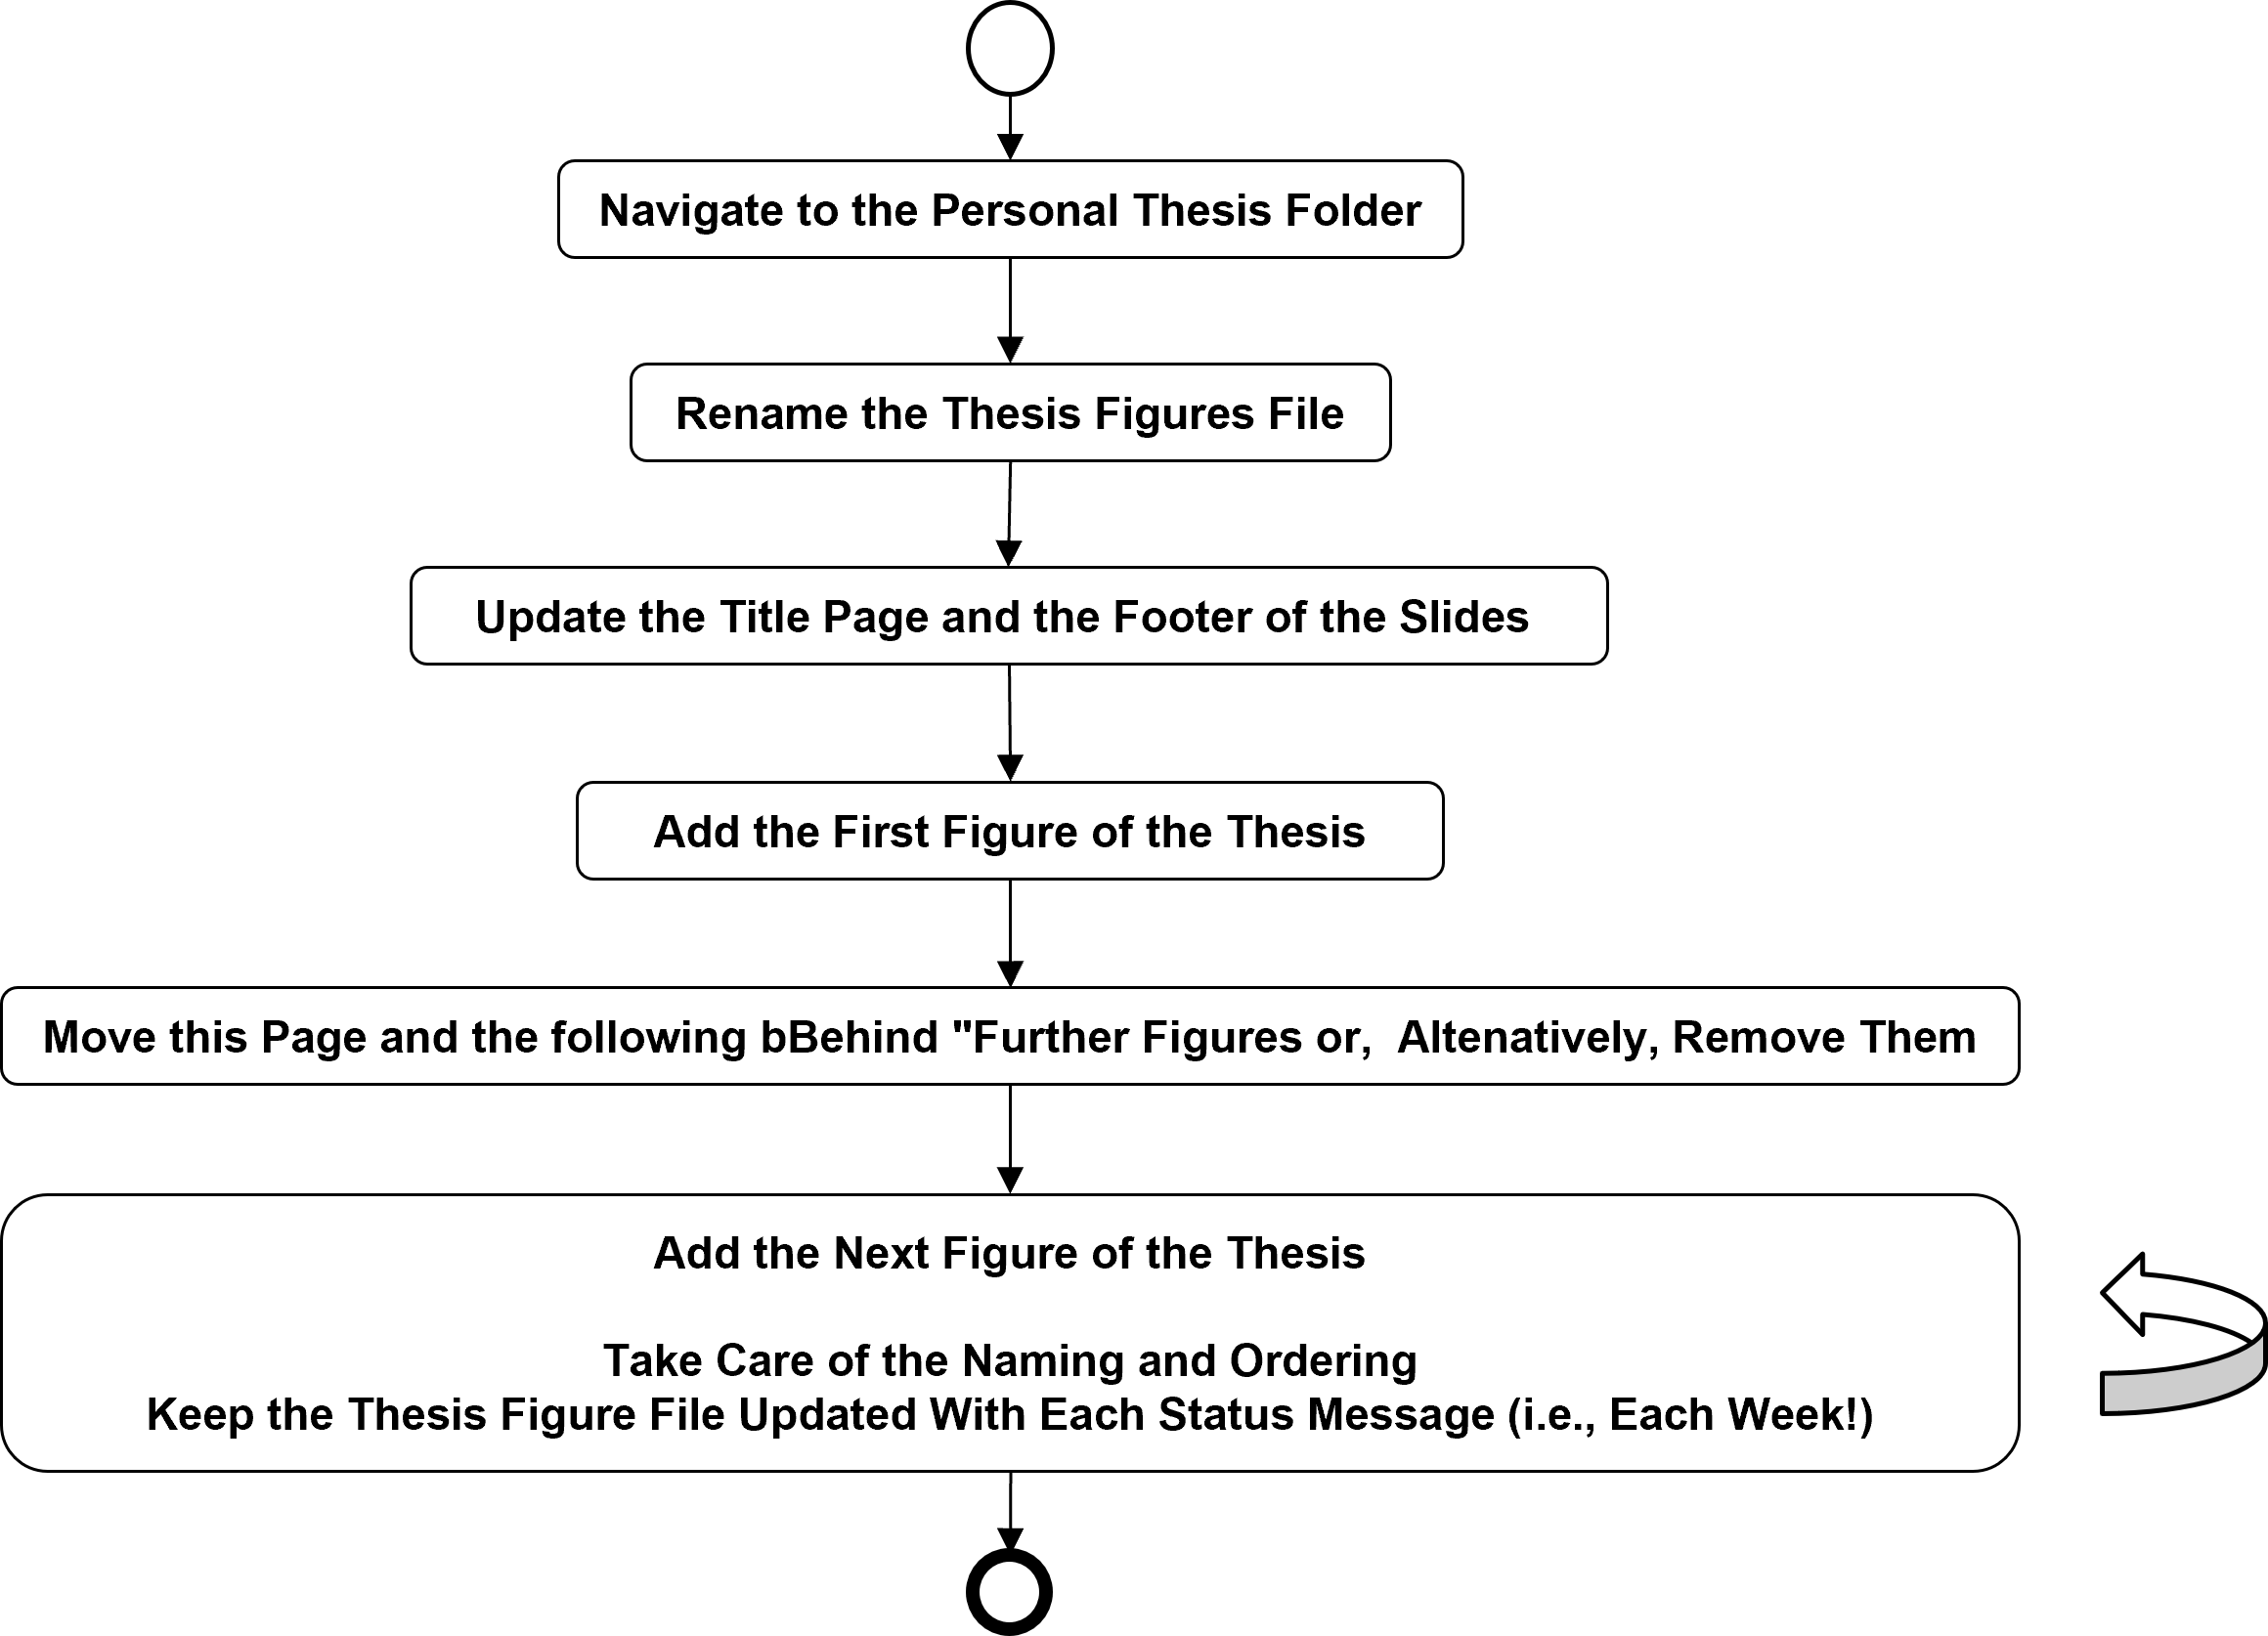
\includegraphics[width=0.8\textwidth]{figures/the_fig_fil_pro.png}
% 	\caption{Thesis Figures File Process}
% 	\label{fig:the_fig_fil_pro}
% \end{figure}

% The steps of the process described in Figure \ref{fig:the_fig_fil_pro} should be carried out by each JuniorStudent
% and SeniorStudent when creating the initial version of the thesis document.

% \subsection{Inserting UML Diagrams}
% UML diagrams are exclusively created with the tool UMLet. The UMLet files are to be stored in the subfolder ``6.UMLet\_Sources''.
% The UMLet diagram is inserted in the format .png in the thesis figures file. The UMLet diagram illustrated in Figure \ref{fig:exa_sys_arc}
% is taken from the WASA lecture.

% \begin{figure}[ht]
% 	\centering
% 	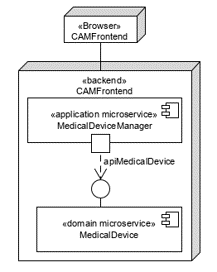
\includegraphics[width=0.4\textwidth]{figures/exa_sys_arc}
% 	\caption{Example of a SystemPlusSoftware Architecture}
% 	\label{fig:exa_sys_arc}
% \end{figure}

% The naming convention of the UMLet file is <figure\_number>.<tite\_of\_the\_figure> as can be easily understood when taking
% a closer look to the folder ``6.UMLet\_Sources'' in which the example diagram shown in Figure \ref{fig:exa_sys_arc} is stored.

% \subsection{Citations}
% \label{subsec:citations}
% Citations can be included in the thesis in the following way:

% \begin{quote}
% \textit{``A microservice is a cohesive, independent process interacting via messages''}
% \end{quote}
% \begin{quote}
% \textit{``fictive book quote.'', \cite[P.~99]{Be02}}
% \end{quote}

% \subsection{Writing Cucumber Features in LaTeX}
% Features are included in the LaTeX code as a special listing and referenced in the text using the feature \ref{lis:example} command.

% \vspace{0.5cm}
% \begin{lstlisting}[caption = {Example for Development Artifacts in the Thesis}, label = {lis:example}, style = kit-cm, language=] 
% First line of the development artifact
% Second line of the development artifact
% \end{lstlisting}

% \subsection{Inserting Tables}
% Table \ref{tab:example_table} shows an simple example for inserting a table in LaTeX.
% \begin{table}[H] 
%Hint: The [H] is part of the packet float. It stands for ``Here'' which means that the table is placed where it is defined.
% 	\centering
% 	\begin{tabular}{ | l | p{7cm} | }
% 		\hline
% 		\textbf{Heading} & \textbf{Further Heading} \\
% 		\hline
% 		 Entry & Example of an entry \\
% 		\hline
% 		 Entry & Example of a further entry \\
% 	 	\hline
% 	\end{tabular}
% 	\caption{Example of a Table}
% 	\label{tab:example_table}
% \end{table}

% \subsection{Linguistic Conventions in the Context of the C\&M Software Development Process}
% All artifacts created during the C\&M software development process are written in English.
% This also applies to the features created in the analysis phase, since it is assumed that the user of a software system
% developed by C\&M is an English speaker. American English is used throughout the thesis.

% An important quality aspect to be considered in software development is the consistent spelling of the introduced terms during development.
% Two levels must be distinguished here: The level of ("natural", English) language and the level of (formal, development-related) artifacts.
% An example of a term at the language level is "Todo List Management".
% As a C\&M convention that terms are written on the artifact level in the so-called CamelCase notation, in this example "TodoListManagement".

\chapter{Foundations}
\label{cha:foundations}

\todo{Add chapter introduction}

\section{Decentralized Identities}
\todo{continue writing}

Decentralized Identities are best explained with an example of how and where they are used.
Alice is a citizen who wants to rent a car. Alice has a decentralized identifier (DID) which is a digital identity
that uniquely identifies her. She also has a digital wallet associated with her DID that she can use
to store digital credentials. Bob is a clerk for a driving license authority.
In order for Alice to be able to rent a car online, she needs a method of proving that she has a valid
driver's license. She goes to Bob and asks him to issue her a Verifiable Credential (VC) for her driving
license, which she could use as proof of her possessing a valid driver's license.
Bob verifies that Alice has a valid driver's license and then issues her the VC using her DID.
The VC is stored in Alice's digital wallet which only she has access to.
When she now goes through the process of renting a car online, the rental company
can ask her to provide a VC to prove that she has a valid driver's license.
Alice can then share her VC from her wallet with the rental company, which can then be
verified through the Trust System. The rental company now knows that Alice has a valid driving license
because they could verify that the VC was valid and associated with Alice's DID.
Alice can now proceed with renting a car online from the rental company.

Throughout this entire process, Alice was in charge of her personal information while
the rental company was still able to verify her possession of a driving license. This is because
the rental company trusts the driving license authority and the Trust System.
An identity system like this that is based upon trust towards certain entities which uses DID's and VC's is called
a decentralized identity system.

The World Wide Web Consortium (W3C) provides a standard for this type of system in their Decentralized Identifiers (DIDs) v1.0
Standard along with the Verifiable Credentials Data Model v1.1 Standard.


\section{Observability and Monitoring}

In 1960, Kalman defined a system to be observable if its exact state at any time can be completely determined
by its outputs \cite{OnTheGeneralTheoryOfControlSystems}. Based on this definition, observability
for modern cloud systems is the practice of capturing outputs from a software system to
infer knowledge about its state. According to Usman et al. observability consists of capturing
three main types of data from a system: logs, metrics and traces, these are often called the
three pillars of observability \cite{ASurveyOnObservabilityOfDistributedEdgeContainerBasedMicroservices}.

\todo{Explain logs, metrics and traces}

Monitoring is defined by the Cambridge Dictionary as
\enquote{to watch and check a situation carefully for a period of time in order to discover something about it}
\cite{CambridgeDictionary}.
For software systems, monitoring 
\enquote{is the process of collecting, analyzing, and using information to track a program's progress toward reaching its objectives and to guide management decisions}
\cite{DynatraceBlog}.

\todo{Cleanup and actually write this section}

% According to \cite{9837035}, observability consists of three pillars: Metrics, Logs, and Traces.
% Metrics.
% Logs are streams of textual information emitted by an application. They can contain information about important
% events, like an incoming request, or provide details about the occurrence of exceptions.
% Traces are a way of tracking the path of requests through a system. A trace contains detailed information
% about all the services that were called during the processing of a request and can be thought of
% as a stack trace for microservices.

% Because of the scope of this work, only Metrics will be used. Logs and Traces will still be considered
% in the development of a solution so that they may be added in the future.

% Because of the scope of this work, only the pillar of Metrics is considered.

% \begin{quote}
% \textit{``Metrics are numerical representations of data that Ops teams use to determine the overall behavior of a system, service, or network component over time.'', \cite{9837035}}
% \end{quote}

% The four golden signals \cite{Beyer2016-xi}
% \begin{itemize}
%     \item Latency: time to service a request
%     \item Traffic: requests per second
%     \item Errors: rate of failed requests
%     \item Saturation: how saturated are constrained resources like memory or I/O
% \end{itemize}

% White-box vs. Black-box Monitoring \cite{Beyer2016-xi}
% \begin{itemize}
%     \item White-box: Monitoring based on internal system metrics.
%     \item Black-box: Monitoring based on externally visible behavior.
% \end{itemize}

% Internal vs. External resources in a monitoring context:
% Internal resources describe resources that allow direct access to their internals.
% An example of an internal resource is a self-hosted microservice.
% External resources describe resources that do not allow direct access to their internals.
% An example of an external resource is a Software-as-a-Service (SaaS) product which is used in a context that should be monitored.

% External resources can, because of their nature, only be monitored using the Black-box approach.
% Internal resources however can be monitored with both the White-box and Black-box approach.

% Motivations for monitoring cloud applications \cite{6483656}
% \begin{itemize}
%     \item Capacity and Resource Planning
%     \item Capacity and Resource Management
%     \item Data Center Management
%     \item SLA Management
%     \item Billing
%     \item Troubleshooting
%     \item Performance Management
%     \item Security Management
% \end{itemize}

% \todo{Capacity and Resource Planning}

% \todo{Capacity and Resource Management}

% Data Center Management is mainly concerned with the efficient usage of resources.
% One key measurement of the efficiency of a data center is its energy efficiency.

% SLA Management refers to the monitoring of parameters, which are defined in Service Level Agreements (SLA).
% These parameters must be within set bounds for an SLA to be considered fulfilled.

% Billing refers to the monitoring of parameters that influence the cost of running an application.
% When an application is hosted on a cloud provider's Infrastructure-as-a-Service (IaaS) system,
% one of those parameters might be the number of compute instances that an application uses.

% While Troubleshooting usually refers to the tracing of requests and failures to provide a dataset for analyzing and fixing issues in an application,
% Monitoring can also be used to aid in troubleshooting by recording the number of failed requests and their context.

% \todo{Performance Management}

% \todo{Security Management}

\section{DevOps}

\todo{Explain DevOps}
\todo{Crossplane}

\chapter{State of the Art}
\label{cha:state_of_the_art}

This chapter contains descriptions of the three most relevant papers for this thesis that are related to the topic
of monitoring in the context of microservices and cloud applications. In Section \ref{sec:cm_literature}
the three papers are sorted into the C\&M LITERATURE with a brief description of their content
and why they should be included in the C\&M LITERATURE. Section \ref{sec:uf+22}
contains a more detailed description of the paper that is most relevant to this thesis
and how it was used in this thesis.

\section{Analysis of and Contributions to the C\&M Literature}
\label{sec:cm_literature}

The C\&M LITERATURE is a list of publications that is maintained by the C\&M research group.
The publications contained in this list are relevant to the different areas of research of the group.
The list is split into five topics. Figure \ref{fig:categories_subcategories} shows an overview of these five categories and
sorts the three papers, described in this section, into these categories. The first topic is Engineering which contains publications
by the C\&M research group itself as well as publications that relate to the different phases
of the general software development process. The second topic is Analysis, Architecture, and Testing.
This topic contains publications that are relevant for modeling software and testing it.
The third topic, Authorization and Policies, focuses on access control for microservice-based applications.
The fourth topic, CI/CD and DevOps, contains publications related to the DevOps concept,
cloud-based software, and observability. Lastly, the fifth topic contains a mix of different publications
that were deemed relevant for the C\&M LITERATURE but do not fit into the other topics.

\begin{figure}[tb]
    \centering
    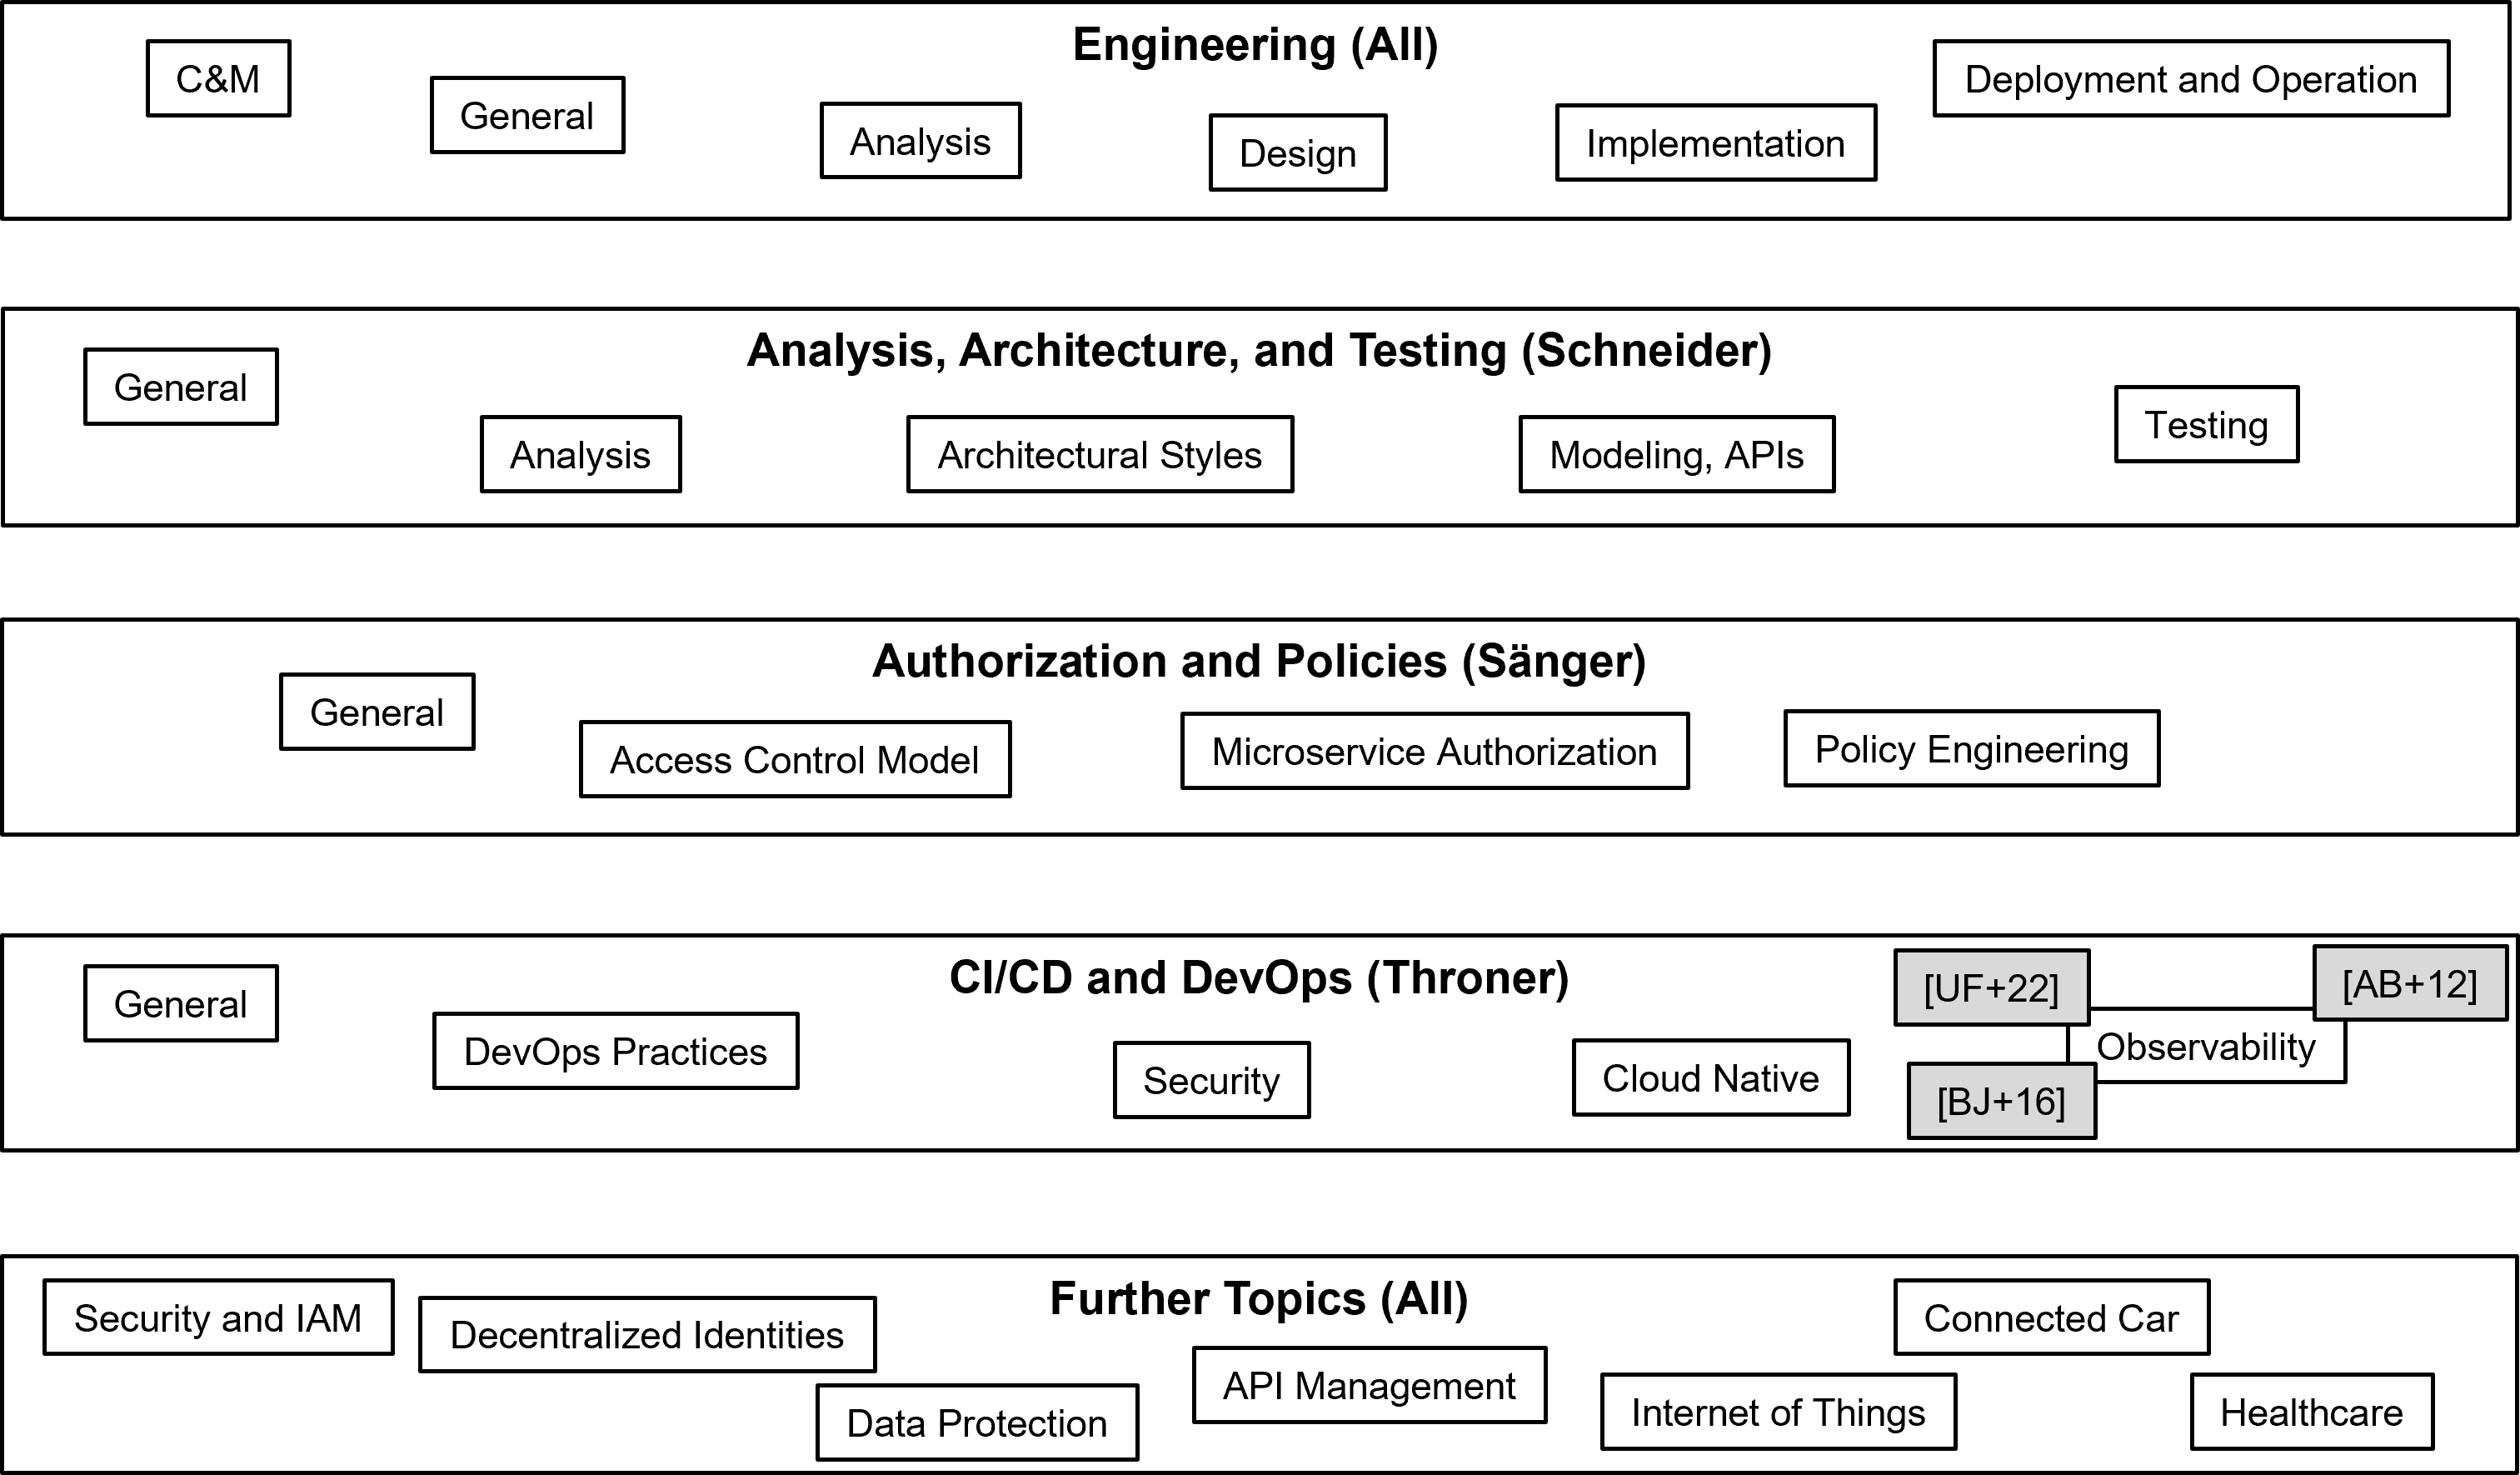
\includegraphics[width=\linewidth]{figures/literature.png}
    \caption{Categories and Subcategories}
    \label{fig:categories_subcategories}
\end{figure}

\subsection*{A Survey on Observability of Distributed Edge \& Container-Based Microservices \cite{UF+22}}

This paper provides a survey of state-of-the-art monitoring solutions.
The paper surveyed different monitoring solutions from academic papers as well as
commercial options. The monitoring solutions were analyzed regarding their scope,
their structure (multi-tenant and multi-layer), the instrumentation they provide (metrics, logs, and tracing),
and whether they are open-source solutions or not. The survey is summarized in a large table
which is followed by a description of each monitoring solution that was surveyed.
Additionally, the paper defines the data needed by an observability system, its basic functionalities,
and its key characteristics. For the context of C\&M, the paper provides a good overview of
both academic and commercial monitoring systems which can be used to investigate
different monitoring solutions in the future.

Status: CREATE (the publication should become a part of the C\&M LITERATURE  (09.09.2023))

\subsection*{Site Reliability Engineering \cite{BJ+16}}

This book by Beyer et al. \cite{BJ+16} discusses how Google develops reliable software
at some of the largest known scales. The authors of the book work in the Site Reliability Team
at Google. Site Reliability Engineering is the practice of using automated tooling
to increase the reliability of large-scale software systems.
The book is divided into five parts. The first part, introduction, introduces
the basic concepts needed by the rest of the book. In the second part, principles,
the book discusses seven principles on which the work of the Site Reliability Team
at Google is based. Part three, practices, goes into detail on the various tasks
of the Site Reliability Team which range from testing and monitoring to incident management.
Part four, management, explains the management aspects of running a Site Reliability Team.
Part five, conclusions, lists lessons learned from other industries and concludes the book.
For the context of C\&M, the book provides interesting insights into large-scale cloud software
systems which are mostly kept as close company secrets. 

Status: CREATE (the publication should become a part of the C\&M LITERATURE  (09.09.2023))

\subsection*{Cloud monitoring: Definitions, issues and future directions \cite{AB+12}}

This paper by Aceto et al. \cite{AB+12} discusses the motivation for monitoring cloud applications
as well as basic concepts and definitions of cloud monitoring. The paper starts by defining
eight tasks of cloud computing for which monitoring is required. This is followed by describing
cloud architecture as consisting of seven layers. Then eight properties are proposed that
a cloud monitoring system should possess. Finally, the paper reviews open issues and future
directions for the research into cloud monitoring. For the context of C\&M,
this paper provides some fundamental definitions for the area of monitoring cloud applications.

Status: CREATE (the publication should become a part of the C\&M LITERATURE  (09.09.2023))

\section{Usman et al.: A Survey on Observability of Distributed Edge \& Container-Based Microservices}
\label{sec:uf+22}

The paper A Survey on Observability of Distributed Edge \& Container-Based Microservices by Usman et al. \cite{UF+22}
was used by this thesis as an entry point into the topic of monitoring cloud-based software.
The paper discusses some of the fundamentals of monitoring like the three pillars of observability
and the four golden signals. Additionally, this paper defines the basic functionalities and key characteristics of an observability system.
While these definitions were not used as explicit goals for the development of the monitoring system in Chapter \ref{cha:first_solution},
they were used as guidelines during the development of the monitoring system and guided different decisions.

While the paper provides important fundamentals for monitoring and observability in general, the key goal of the paper
was a survey of modern observability solutions both from academia and the industry.
In total, the paper compared 43 different solutions based on their scope, whether they support multi-tenancy or multi-layer observability,
which pillars of observability are captured by the solutions and if they are open source or not.
This list was used as a basis for selecting the different components of the monitoring system developed in Chapter \ref{cha:first_solution}.


\chapter{Overall Concept of the Developed Solutions}

% In this first result chapter of the thesis the overall concept which clarifies the relationship of the investigated issues is introduced. From this overall concept all further result chapters and the solutions covered by each of these chapters should be derived.

\chapter{Technical Foundation}

% In this chapter, the technical foundation of the solutions developed in this thesis is worked out. Usually, this is the first chapter written by each SeniorStudent since it describes the current (technical) status the further work of this thesis is based on. By doing so, the continuity of the work carried out by the research group C\&M is guaranteed. Additionally, this chapter deals for those JuniorStudents who are co-supervised by the SeniorStudent (the author of this thesis) as one of the most relevant sources for the JuniorStudents' practical work.

% Depending on the concrete topic of the thesis, the technical foundation may include the (i) software and/or system architecture of the software system under investigation, (ii) the artifacts relevant for the thesis, (iii) tools that are applied, (iv) any further technical system or solution. These parts of the technical foundation should be described from the viewpoint of the specific topic of this thesis. For example, if an artifact is relevant for the topic, only the topic-related aspects of this artifact (and not just the artifact) should be illustrated in this chapter.

% General description of concepts or solutions are NOT part of this chapter, but should be transferred to other chapters of the thesis (e.g., Chapter 1 or Chapter 2). This also holds for the description of concrete solutions which are NOT to be described in Chapter 5 but in the following chapters. The focus of Chapter 5 is to make clear what is missing in the current technical solution in order to motivate the work which will be carried in this thesis (and which will be further described in the following chapters).

% Relevant sources for the content of Chapter 5 are: (i) WASA lecture, (ii) latest Bachelor/Master/PhD theses, (iii) latest publication. The WASA lecture contains the current and, therefore, the ``valid version'' of concepts and solutions. So this content should be trusted if there is a mismatch between WASA lecture and theses or publications.


\chapter{SPMonitor}

% This is the third result chapter which presents the first solution of the thesis.
% The solution is integrated into the overall concept introduced in Chapter 4 and
% it is technically based on the foundation described in Chapter 5.

% A thesis should provide at least two such solutions.

\todo{Add chapter introduction}
\todo{Explain purpose: maybe move motivation here; away from Analysis}

This chapter will focus on the development of SPMonitor.

\subsection{Motivation}
The DrivingLicenseAuthorityKarlsruhe (DLAKa) wants to provide citizens with digital driving licenses,
which can, for example, be used to prove to a car rental company that they possess a valid driving license.
They hire the company ServiceProvider (SP) to develop and operate the system necessary for issuing and verifying
digital driving licenses. The contract specifies an initial payment for the development of the system
and afterward a yearly fee for the operation of the system.
After receiving the contract from DLAKa, SP starts designing the system
for DLAKa. Because SP has to operate the system on a fixed yearly budget,
they want to monitor the performance of the system to identify parts with excessive resource usage, which
incur additional costs. They identify the CPU and memory usage of the system as two technical metrics that should be monitored.
Additionally, DLAKa has asked them to provide the capability of monitoring business metrics for them.
DLAKa wants to know how many digital driving licenses are being issued and how often the issuance of a digital
driving license fails. To monitor both technical and business metrics, SP designs the ServiceProviderMonitor (SPMonitor) as a part
of the system for DLAKa which will provide all functionality for monitoring the specified metrics.

BestRental, a car rental company, has heard of DLAKa's plans for digital driving licenses
and wants to integrate them into its online rental system. Contrary to DLAKa, BestRental develops its
system in-house. Similarly to DLAKa, BestRental is interested in obtaining business metrics from its system.
They want to use these metrics to make business decisions like if they should increase the capacity of their fleet in the future.
For this purpose, BestRental designs an additional application called BestMonitor that will provide all the monitoring functionality.
In the beginning, they are only interested in one metric: How many active rentals are there?

For the design of SPMonitor, SP created two use cases: Present Metric and Collect Metric.
The relation of these use cases can be seen in the Use Case Diagram in Figure \ref{fig:use_case_monitoring_dlakaapp}.
Present Metric handles the use case of presenting the collected metrics to a user, this is described in Listing \ref{lis:use_case_description_present_metric}.
Collect Metric is concerned with how SPMonitor receives metrics for later presentation to a user, this is described in Listing \ref{lis:use_case_description_collect_metric}.

The metrics that will initially be monitored by SPMonitor are the number of issued digital driving licenses (NumDDL)
and the memory usage of the DLAKaApp (MemUse). The NumDDL metric is a business metric for DLAKa, while MemUse is
a technical metric that allows SP to monitor the performance of DLAKaApp.

\section{Analysis}

\todo{Introduction to Analysis}

\begin{figure}
	\centering
	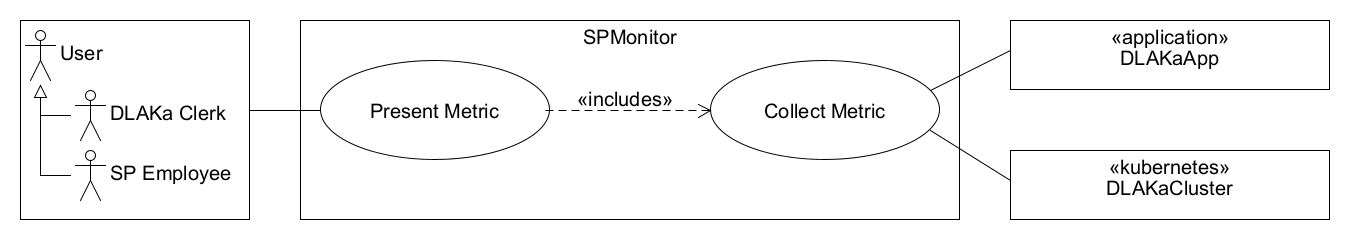
\includegraphics[width=\textwidth]{figures/2.1_use_case_spmonitor.png}
	\caption{Use Case Diagram: SPMonitor}
	\label{fig:use_case_monitoring_dlakaapp}
\end{figure}

\subsection{Use Case Present Metric}
\todo{Elaborate}

\begin{lstlisting}[caption = {Use Case Description: Present Metric}, label = {lis:use_case_description_present_metric}, style = kit-cm, language=]
Title: Present Metric

Primary Actors: DLAKa Clerk

Preconditions:
- SPMonitor has the NumDDL metric configured

Flow:
1. DLAKa Clerk opens the dashboard for the NumDDL metric
2. SPMonitor retrieves all stored values for the NumDDL metric
3. SPMonitor displays the values in a graph

Alternative Flows:
2a. SPMonitor has no values stored for the NumDDL metric
2a1. SPMonitor displays a message that the NumDDL metric has no stored values

Information Requirements:
- Values for the NumDDL metric
\end{lstlisting}

\subsection{Use Case Collect Metric}
\todo{Elaborate}

\begin{lstlisting}[caption = {Use Case Description: Collect Metric}, label = {lis:use_case_description_collect_metric}, style = kit-cm, language=]
Title: Collect Metric

Secondary Actors: DLAKaApp, DLAKaCluster

Preconditions:
- DLAKaApp is set up to collect the NumDDL metric
- DLAKaCluster is set up to collect the MemUse metric
- DLAKaApp is running inside of the DLAKaCluster
Postconditions:
- SPMonitor has values stored for NumDDL and MemUse

Flow:
1. SPMonitor sends a request to DLAKaApp for the NumDDL metric
2. DLAKaApp replies with a value for the NumDDL metric
3. SPMonitor receives the reply
4. SPMonitor stores the value for the NumDDL metric
5. SPMonitor sends a request to DLAKaCluster for the MemUse metric
6. DLAKaCluster replies with a value for the MemUse metric
7. SPMonitor receives the reply
8. SPMonitor stores the value for the MemUse metric

Alternative Flows:
2a. DLAKaApp replies with an error message
2a1. SPMonitor receives the error message
2a2. SPMonitor retries to request the NumDDL metric
6a. DLAKaCluster replies with an error message
6a1. SPMonitor receives the error message
6a2. SPMonitor retries to request the MemUse metric

Information Requirements:
- Value for the NumDDL metric
- Value for the MemUse metric
\end{lstlisting}

\todo{Summarize Analysis}

\section{Design}

\todo{Introduction for Design}

\subsection{Metrics Definition}

\subsection{Selecting the Tools}

As explained in Chapter \ref{cha:technical_foundation}, a monitoring system consists of three parts:
The Data Source, Data Sink and a tool for visualization.
The data source is the core of a monitoring system. It is responsible for collecting the monitoring data
and dictates the needs for the data sink as well as the possibilities for the visualization.
Because of its central role, the data source will be the first component of the monitoring system that will be chosen
and the rest of the monitoring system will be chosen to best fit with and support the data source.

In order for the chosen data source to best fit the needs of SPMonitor, it needs to fulfill some requirements
which stem from SPMonitor's use cases. The first requirement for the data source is that it should be built
to support the use cases of SPMonitor. Tools that are built for different purposes but could be used for SPMonitor's
use cases, will be less preferable than tools that are designed for SPMonitor's use cases.
Secondly, the data source should be free to use. This requirement mostly stems from the scope of this work
as a bachelor's thesis without any funding.
Additionally, the data source needs to be able to collect technical metrics as well as business metrics.
While technical metrics can be gathered from most cloud environments automatically, business metrics
require the instrumentation of the source code of the monitored services. Many data sources can in theory
instrument service but they often use additional tools like OpenTelemetry for this. Because SPMonitor aims
to be as slim as possible, to reduce complexity, data sources that can instrument services on their own without
the need for an additional tool, will be preferred over data sources that can not do that.
Lastly, the data source needs to support two different cloud environments: Kubernetes for the on-premise parts
of DLAKaApp and Microsoft Azure for the decentralized identity part of DLAKaApp.

These six requirements for the data source are listed in Table \ref{tab:data_source_requirements}.
Requirements R2 through R6 are hard requirements, meaning that a data source that does not fulfill them
will not be chosen. Requirement R1 is a soft requirement that is meant as an orientation and does directly
lead to the elimination of a data source.

\begin{table}[]
\centering
\begin{tabular}{c|l}
Key & Requirements \\
\hline
R1 & Purpose \\
R2 & Licensing \\
R3 & Technical metrics \\
R4 & Business metrics \\
R5 & Kubernetes \\
R6 & Microsoft Azure \\
\end{tabular}
\caption{}
\label{tab:data_source_requirements}
\end{table}

The data sources that will be compared according to the requirements in Table \ref{tab:data_source_requirements} stem
from the paper \enquote{A Survey on Observability of Distributed Edge {\&} Container-Based Microservices}
by Usman et al. \cite{ASurveyOnObservabilityOfDistributedEdgeContainerBasedMicroservices}. The list from that survey was supplemented with one additional entry,
the TICK (Telegraf, InfluxDB, Chronograf, Kapacitor) stack. Any entries that do not support metrics or are purely research projects were eliminated.
Lastly, the entry for Kibana was changed to ELK for the ELK (ElasticSearch, LogStash, Kibana) stack.
The complete overview of all analyzed tools can be seen in Table \ref{tab:data_source_comparison}.

\begin{table}[]
\centering
\begin{tabular}{l|c|c|c|c|c|c}
Name & R1 & R2 & R3 & R4 & R5 & R6 \\
\hline
Apache SkyWalking		 & Performance & Free & \cmark & \cmark & \cmark & \xmark \\
Cilium					 & Networking & Free & \cmark & \xmark & \cmark & \cmark \\
Datadog					 & SaaS & Paid & \cmark & \cmark & \cmark & \cmark \\
Dynatrace				 & PaaS & Paid & \cmark & \xmark & \cmark & \cmark \\
ELK						 & Searching & Paid & \cmark & \xmark & \cmark & \cmark \\
Honeycomb				 & Debugging & Paid & \cmark & \cmark & \cmark & \cmark \\
Instana					 & Incidence Management & Paid & \cmark & \xmark & \cmark & \cmark \\
Monasca					 & MaaS & Free & \cmark & \xmark & \cmark & \xmark \\
New Relic				 & PaaS & Paid & \cmark & \cmark & \cmark & \cmark \\
\rowcolor{lightgray}
OpenTelemetry			 & Monitoring & Free & \cmark & \cmark & \cmark & \cmark \\
\rowcolor{lightgray}
Prometheus				 & Monitoring & Free/Paid & \cmark & \cmark & \cmark & \cmark \\
Scalyr					 & PaaS & Paid & \cmark & \xmark & \cmark & \xmark \\
SolarWinds				 & PaaS & Paid & \cmark & \xmark & \cmark & \cmark \\
Splunk					 & Resilience & Paid & \cmark & \cmark & \cmark & \cmark \\
Sumo Logic				 & Analytics & Paid & \cmark & \cmark & \cmark & \cmark \\
\rowcolor{lightgray}
TICK					 & Time Series Data & Free/Paid & \cmark & \cmark & \cmark & \cmark \\
\end{tabular}
\caption{Comparison of data sources}
\label{tab:data_source_comparison}
\end{table}

The three final candidates for use in SPMonitor can be seen highlighted in Table \ref{tab:data_source_comparison}.
They are OpenTelemetry, Prometheus, and the TICK stack.
OpenTelemetry is a standalone solution for the collection of metrics. 
It provides many client libraries to instrument service for business metrics and can integrate
with most data sinks and visualization tools.
Prometheus is commonly used in combination with the LGTM (Loki Grafana Tempo Mimir) stack.
Loki is a service for handling logs, Tempo is responsible for handling traces, Grafana is used for visualization and Mimir provides
long-term storage for Prometheus. Prometheus itself is responsible for the collection of metrics.
As this work only considers metrics, the full setup would use Grafana for visualization, Prometheus as the data source, and Mimir
as the data sink. As Mimir only provides Prometheus with an interface to a storage system and is itself not one, it can be paired with MinIO
a free-to-use object storage system.
The TICK stack consists of four different tools: Telegraf, InfluxDB, Chronograf, and Kapacitor.
Telegraf is responsible for collecting metrics from the monitored services. The collected metrics are then forwarded
to InfluxDB, the storage component of the stack, and Kapacitor which is responsible for data processing.
Chronograf provides the interface to visualize and analyze the collected metrics.

From these three options, Prometheus together with Grafana, Mimir, and MinIO was chosen for SPMonitor.
Unlike OpenTelemetry, Prometheus provides easy integration with its data sink and visualization tool as
they were built to work together. OpenTelemetry on the other hand is a standalone solution meant to enhance
other tools which do not collect metrics themselves. The TICK stack provides the same integration benefit compared
to OpenTelemetry. The decision between Prometheus and the TICK stack is not as straightforward.
Both fulfill all requirements, offer extensibility options through plugins for different data sources
and pre-built visualizations, and they are both open-source projects which can be freely used.
One difference between them is that there exists a provider solution for managing Grafana with Crossplane.
This does not seem to exist for the TICK stack. Crossplane will be used to provision and operate the cloud
services of DLAKaApp and SPMonitor. Therefore Grafana and Prometheus are chosen for SPMonitor as they offer tools
for integrating them with Crossplane compared to the TICK stack. The final selection of tools can be seen in Figure \ref{fig:spmonitor_tech_stack}.

\begin{figure}
	\centering
	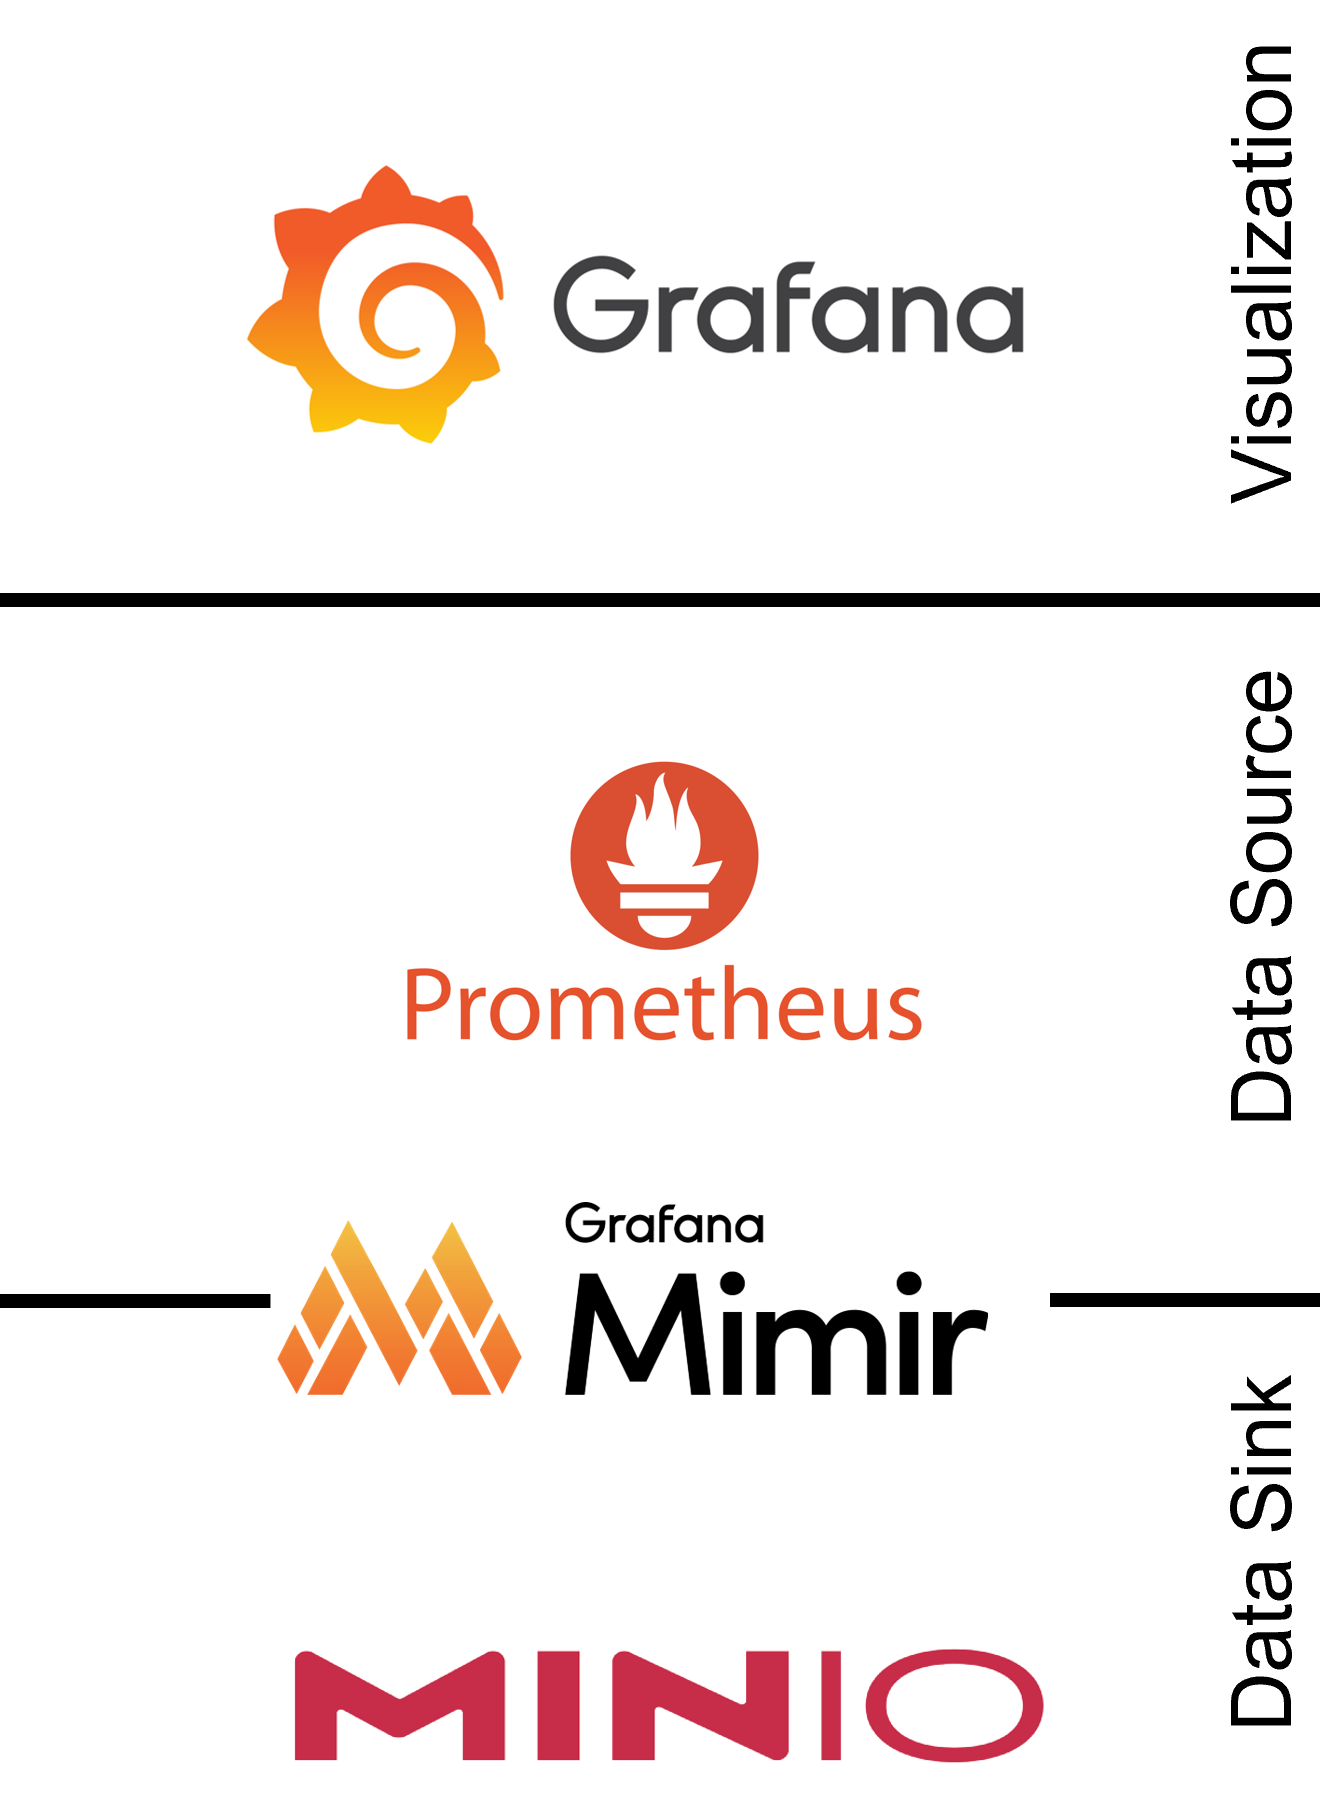
\includegraphics[width=0.4\textwidth]{figures/spmonitor_tech_stack.png}
	\caption{SPMonitor Technology Stack}
	\label{fig:spmonitor_tech_stack}
\end{figure}

\subsection{Architecture}

\todo{Explain SPS Architecture}

\begin{figure}[h]
	\centering
	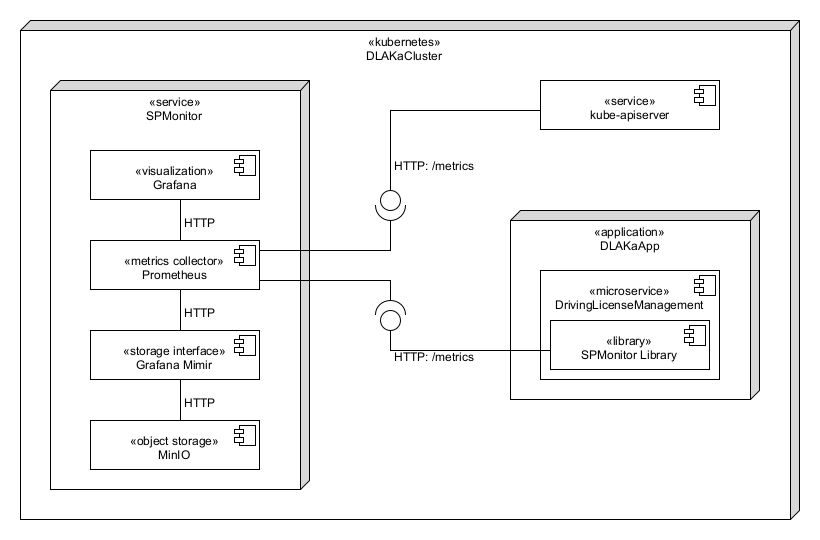
\includegraphics[width=\textwidth]{figures/sps_spmonitor.png}
	\caption{SystemPlusSoftware SPMonitor}
	\label{fig:sps_spmonitor}
\end{figure}

\subsection{API Specification}

\subsection{DevOps Concept}

\section{Implementation}

\chapter{Second Solution (Chapter Title is to be Adapted)}

\todo{Add chapter introduction}

% This is the fourth result chapter which presents the second solution of the thesis. The solution is integrated into the overall concept introduced in Chapter 4 and it is technically based on the foundation described in Chaper 5.


\chapter{Practical Task}

% In this chapter the results of the practical tasks carried out in cooperation with a research partner are reported. The chapter should be self-contained meaning that all relevant aspects of the task, such as the foundation and state of the art of the investigated topics should be an integral part of this chapter.


\chapter{Organization of the Project Team}
\label{cha:projektteam-arbeiten}

\todo{Add chapter introduction}

\chapter{Summary and Outlook}
\label{cha:outlook}

\todo{Add chapter introduction}

%
% add appendix
%

\chapter{Appendix}
\chaptermark{Appendix} 

\section{WASA2 Contributions}

\todo{Add WASA2 lecture contribution}

\section{Snack and Learn}

\todo{Add summary of Snack and Learn}

% \clearpage
\section{Best Practices and Guidelines}

\todo{Add Guideline about Postgres Driver for Go}

% \subsection{Best Practices Template}
% 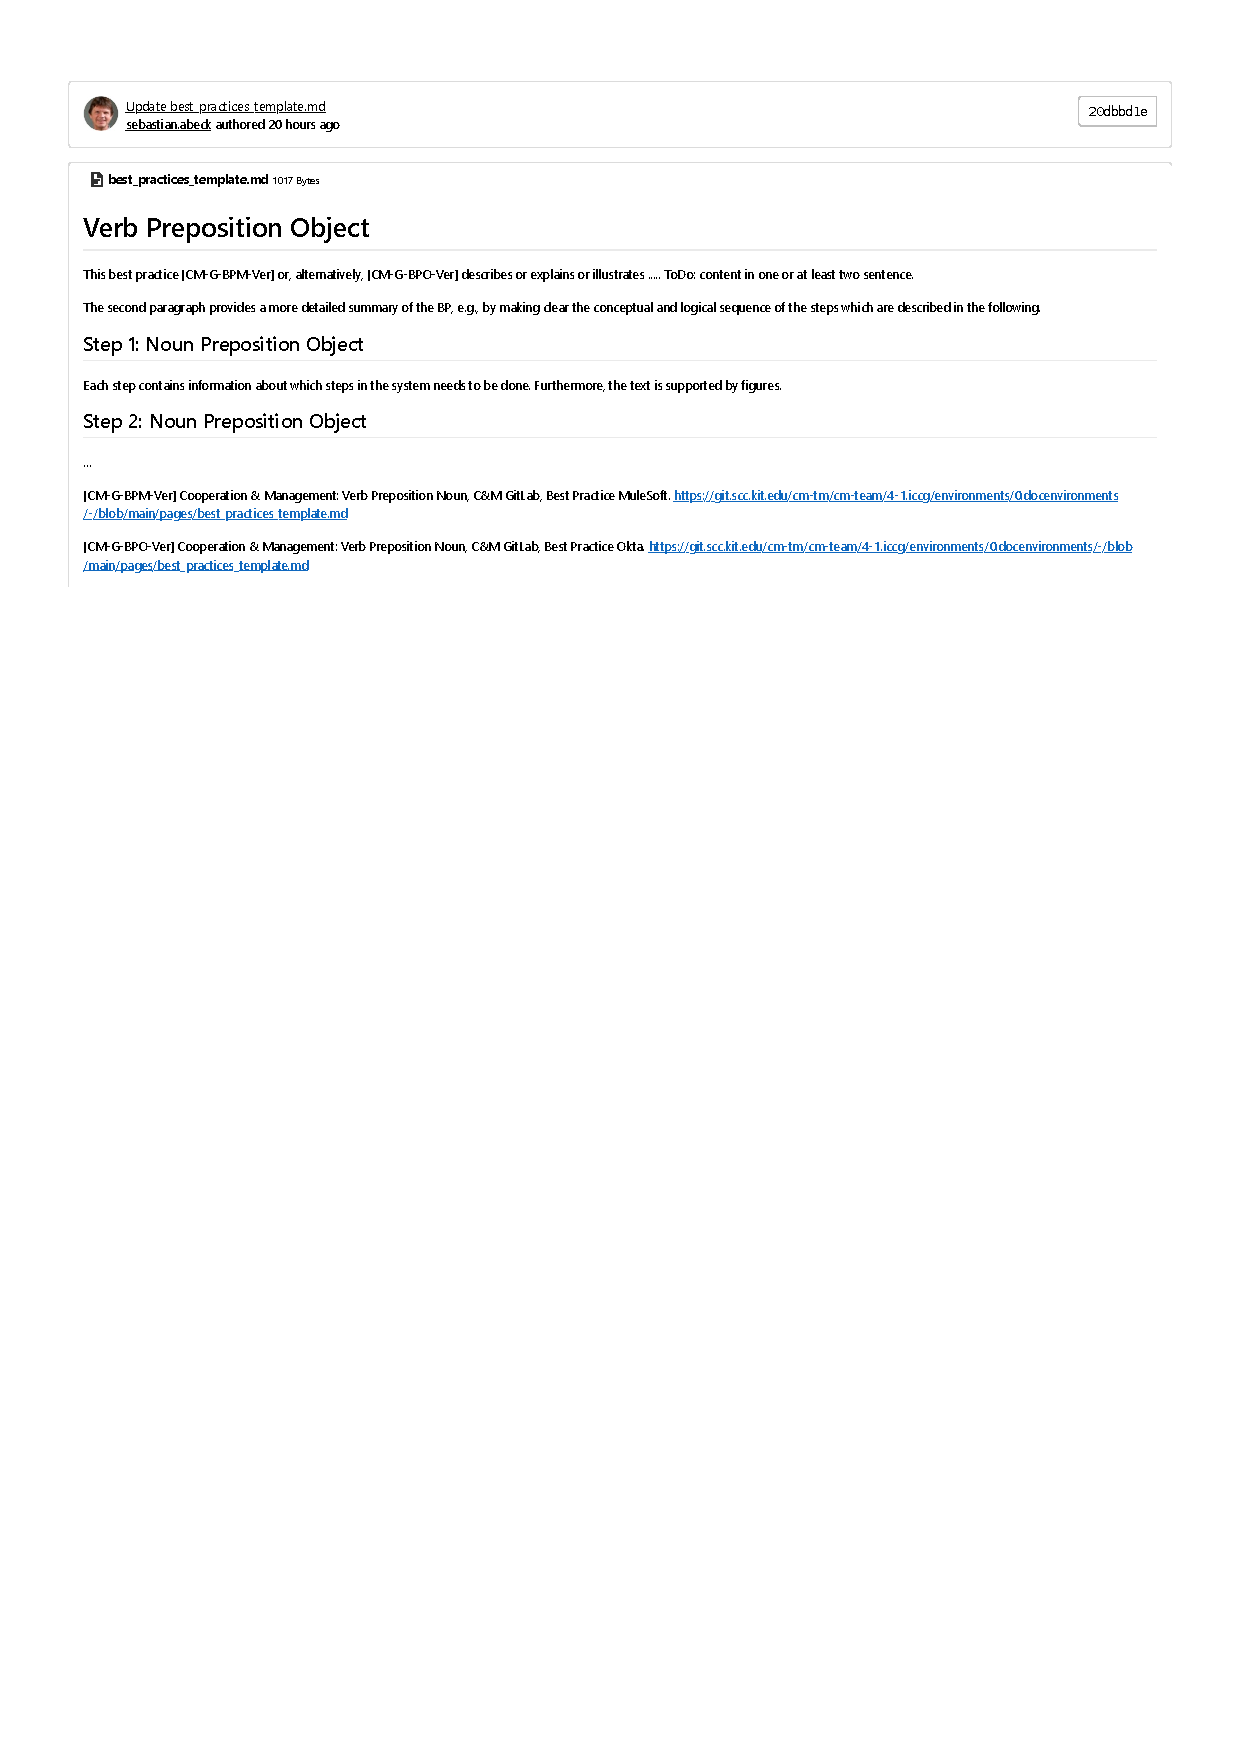
\includegraphics[height=0.9\textheight]{pdfs/b1.best_practice_template.pdf}

% \clearpage
% \section{Miscellaneous}

% \clearpage
% \section{Publication Contributions}


\clearpage


%
% Bibliography
%
\makeatletter
\renewenvironment{thebibliography}[1]
     {\section{\bibname}
      \list{\@biblabel{\@arabic\c@enumiv}}
           {\settowidth\labelwidth{\@biblabel{#1}}
            \leftmargin\labelwidth
            \advance\leftmargin\labelsep
            \@openbib@code
            \usecounter{enumiv}%
            \let\p@enumiv\@empty
            \renewcommand\theenumiv{\@arabic\c@enumiv}}
      \sloppy
      \clubpenalty4000
      \@clubpenalty \clubpenalty
      \widowpenalty4000
      \sfcode`\.\@m}
     {\def\@noitemerr
       {\@latex@warning{Empty `thebibliography' environment}}%
      \endlist}
\makeatother

\bibliography{bt_engbrocks}

\bibliographystyle{cmnat}

\clearpage

\printglossaries

%
% Insert PDFS
%
%\includepdf[pages=1, pagecommand={\section{Abschnitt} \thispagestyle{scrheadings}}, scale=0.7]{pdfs/anhang.pdf}
%\includepdf[pages=2-last, pagecommand={\thispagestyle{scrheadings}}, scale=0.7]{pdfs/anhang.pdf}

%==============================================================================

\end{document}